\chapter{Sintaksna analiza}

\section{Uvod}
Cilj sintaksne analize je provjeriti odgovara li niz leksema gramatičkoj strukturi (pravilima). Produkt
sintaksne analize (parsiranja) je sintaksno stablo. Gramatička pravila su zadana konteksno-neovisnom
gramatikom u BNF obliku.

Postoje razne tehnike parsiranja s raznim karakteristikama: skup jezika koji obuhvaćaju, težina
implementacije, pogodnost za automatsko generiranje parsera iz gramatike itd.

Naš sintaksni analizator gradi stablo tehnikom odozdo prema gore i spada u LR parsere. Tehnika
kojom generira tablicu prijelaza iz gramatike koju koristi parser se naziva LALR.

\section{Implementacija}

U implementaciji smo koristili generator LR parsera CUP koji generira parser napisan u programskom jezik Java.
Parser predstavlja razred \texttt{Parser} čiji konstruktor prima objekt razreda \texttt{Lexer}
kojeg koristi za dohvaćanje leksema.

Parser radi s objektima razreda \texttt{Symbol}. Oni mogu predstavljati završni (leksem) ili nezavršni znak gramatike.
Razred \texttt{Symbol} sadrži atribut \texttt{value} u koji pohranjujemo objekte razreda \texttt{TreeNode}. Razred
\texttt{TreeNode} predstavlja jedan čvor u sintaksnom stablu i čuva listu svoje djece.

U zadnjoj redukciji u nezavršni znak "program", atribut \texttt{value} će sadržavati vrh sintaksnog stabla i parser
će vratiti upravo taj vrh s kojim smo zapravo dobili cijelo stablo.

U CUP-u se osim produkcija zadaju i akcije koje se izvrše prilikom primjene redukcije određene produkcije. Upravo
te akcije koristimo za gradnju stabla pomoću \texttt{TreeNode}-ova.

\section{Gramatika}

Gramatika je dana u obliku kojeg prima CUP i može se vidjeti u dodatku A. Prednost operatora je rješenja pomoću CUP-a tako
da gramatika ostane što jednostavnija.

\section{Primjer izvođenja}
Pogledajmo primjer izvođenja sintaksne analize za sljedeći jednostavni program:

\lstinputlisting[language=C]{primjer-sintaksna1.c}

\begin{figure}[H]
  \centering
    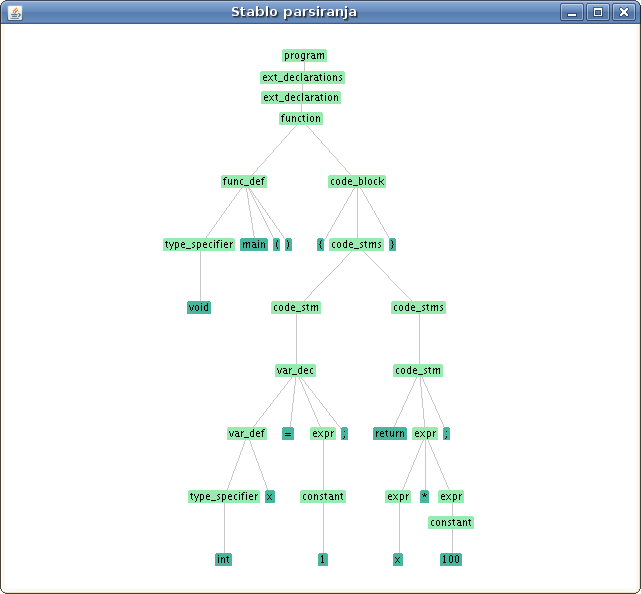
\includegraphics[width=13cm]{primjer-sintaksna1}
  \caption{Primjer izvođenja sintaksne analize}
\label{komponente}
\end{figure}
